\appendix 
\addcontentsline{toc}{section}{Appendix}
\section{Capabilities of the framework}
The framework we implemented for this project has been designed to accommodate an arbitrary number of obstacles. We differentiate two types of obstacles:

\begin{itemize}
    \item static obstacles, which represent extended regions of the road with local parameters that differ from the general set (e.g.\ lower speed limit $v_0$, etc.);
    \item traffic lights, which are point-like obstacles, periodically modulated in time, and disallow any cars to pass during the red phase.
\end{itemize}

\begin{figure}[h!]
    \centering
    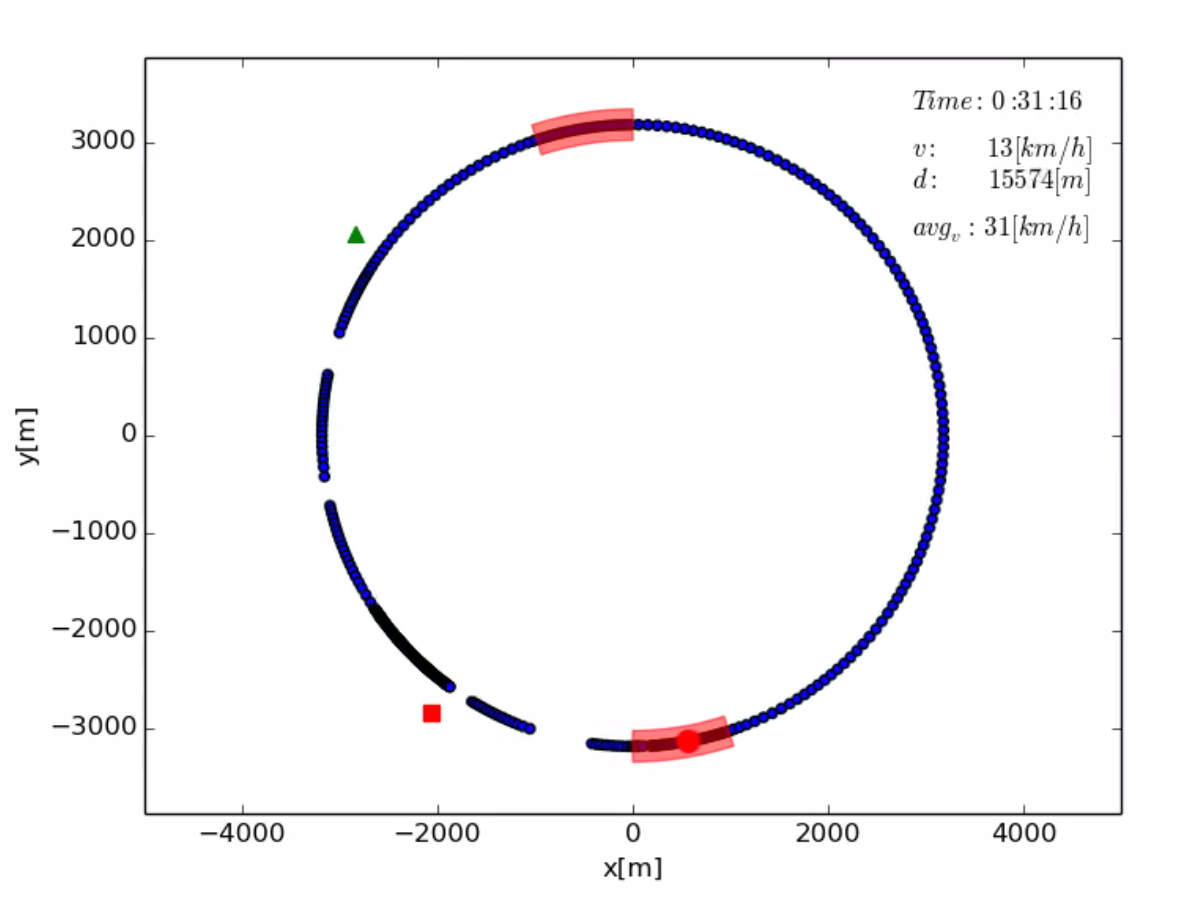
\includegraphics[width=0.7\textwidth]{../img/traffic_light.png}
    \caption{Bird's-eye view of simulated road. The blue markers represent cars (the larger red marker is a reference car for easier visualization). The regions shaded in red are static obstacles, where the speed limit is reduced compared to regular road. The square and the triangle represent traffic lights and their respective state.}
\end{figure}

\noindent The source code of the implementation is available for download from GitHub\footnote{ \url{https://github.com/polwel/traffic_simulation}}.

